\chapter{Empirical Studies}
\label{ch:empirical-studies}

\section{Introduction}
In this section we include the analysis of two of the techniques used in the project: the Viola-Jones method and the Convolutional Neural Networks. In order to prove their effectiveness we will perform an experiment for each of them. The experiments have been fully documented, including the data set used and the results, which are discussed at the end.


%███████╗██╗  ██╗██████╗ ███████╗██████╗      ██╗
%██╔════╝╚██╗██╔╝██╔══██╗██╔════╝██╔══██╗    ███║
%█████╗   ╚███╔╝ ██████╔╝█████╗  ██████╔╝    ╚██║
%██╔══╝   ██╔██╗ ██╔═══╝ ██╔══╝  ██╔══██╗     ██║
%███████╗██╔╝ ██╗██║     ███████╗██║  ██║██╗  ██║
%╚══════╝╚═╝  ╚═╝╚═╝     ╚══════╝╚═╝  ╚═╝╚═╝  ╚═╝

\section{Experiment 1: Effectiveness of Viola-Jones method for Face Detection}
	\subsection{Objective}
	As it was already explained in the Research section (\ref{subsec:face_detec_techniques}), the Viola-Jones method "stands out for performing a high detection rate with a very low false positive rate and it is capable to work in a real time situation". These features have made it widely used in the recent years and it was also the reason why it was finally chosen for this project. 

	\clearpage

	In this experiment, we are going to test this affirmation by applying the method to a certain set of images. It will be composed of an equal proportion of face images, near-face images from a human perspective and non-face images. The results will be displayed including the faces that were correctly detected, the faces that were missed (i.e. false negatives) and the images incorrectly classified as having a face, when they did not (i.e. false positives).

	\subsection{Method and parameters}
	The computer used to run the experiment is a laptop Toshiba C50-A-1GU with a 2,40 GHz Intel Processor Core i3-4000M, 8GB 1600MHz RAM memory and Kubuntu 17.10 OS (Linux kernel version 4.13.0-38-generic). The Viola-Jones method is applied using the OpenCV library as it was done in the \textit{Intelligent Assistant}. In fact, the code used for this experiment (Figure \ref{fig:fd_experiment_code}) is pretty similar to the included in the \textit{face{\_}detection} module, discussed in the Design chapter (\ref{subsec:face_det}).

	\begin{figure}[!ht]
		\centering
		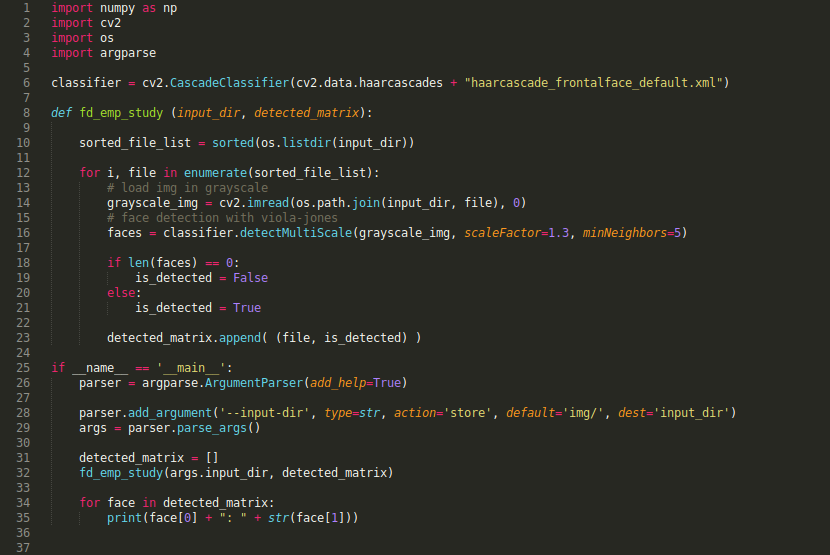
\includegraphics[width=14cm]{emp_studies/fd_experiment_code}
		\caption{Code used to run the Experiment 1}
		\label{fig:fd_experiment_code}
	\end{figure}

	The images are located in a folder named "img", in the same directory as the file. The filename of these images indicates the group to which it belongs and the id of the image, an integer of 2 units filled with zeros if necessary. Then, the filename of the images follow one of these patterns: "face{\_}XX.jpg", "near-face{\_}XX.jpg" or "non-face{\_}XX.jpg".

	The classifier selected for this task is "haarcascade{\_}frontface{\_}default", the same used in the application. The images are loaded in grayscale and the classifier is applied to perform the face detection. This method returns an array with the location of the detected faces in the image, so evaluating its length, we know whether the classifier detected a face or not (i.e. the array would be empty). 

	\subsection{Data set}
	The dataset used in the experiment is composed of a total of 90 images, where 30 of them contain a human face, 30 contain a pattern that humans could interpret as face and 30 do not contain any face. In the Figure \ref{fig:fd_dataset} we can see the complete dataset. All images are square-shaped with a resolution of 250x250 pixels. The face images belong to the \gls{lfw} dataset (\cite{lfw_db}), while near-face images and non-face images were obtained using Google images and after cropped manually.

	The non-face images were obtained after searching for the keys "background" and "abstract wallpaper". The near-face dataset must be explained in detail because the subjective decision of whether the image look like a face enough or not. This group of photos is internally divided in another three sub-groups:

	\begin{itemize}
		\item Images from 1 to 11. The first contain pencil or graphic drawings that represent human faces looking straight forward.
		\item Images from 12 to 20. The second group contain cropped faces from paintings that may have variations in the proportions of some face features. 
		\item Images from 21 to 30. The third and last group contain photos from faces of real sculptures.
	\end{itemize}

	\begin{figure}[!ht]
		\centering
		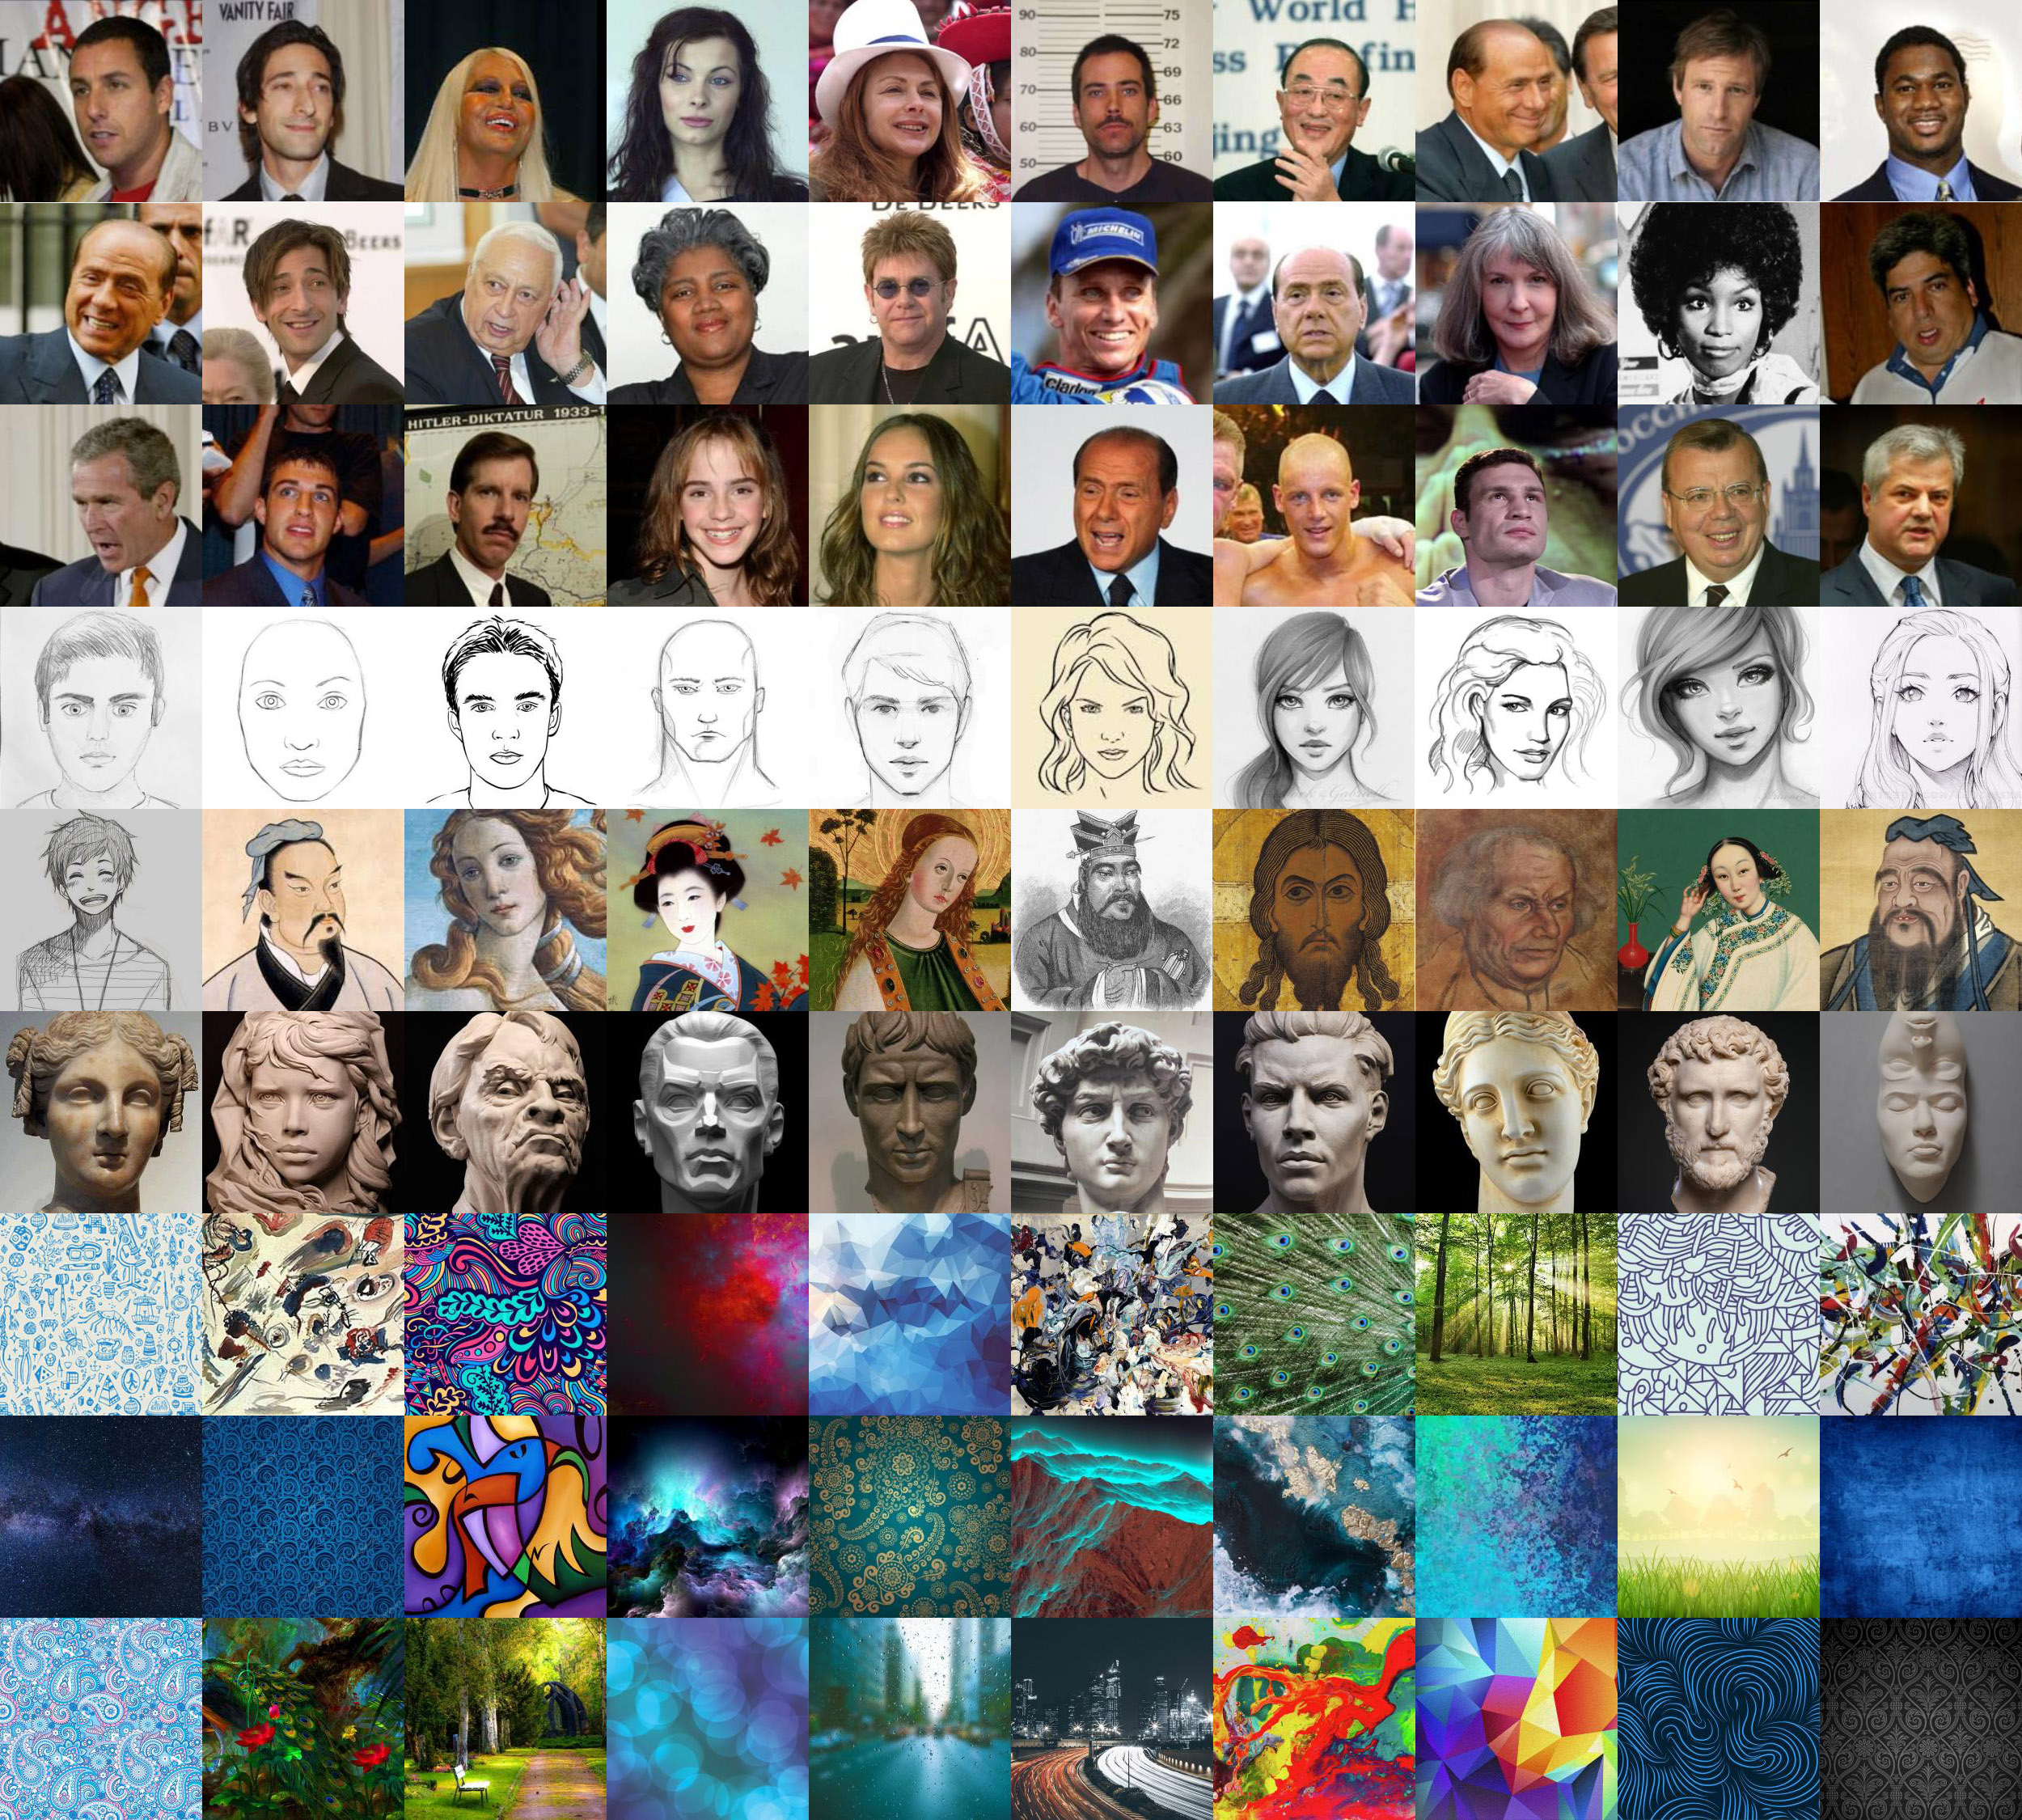
\includegraphics[width=\textwidth]{emp_studies/fd_dataset}
		\caption{Dataset for the Experiment 1}
		\label{fig:fd_dataset}
	\end{figure} 

	\subsection{Results}
	The results of the experiment are shown in Figure \ref{plot:results_exp1} and in the Table \ref{table:experiment_1_res}, where the rows refer to the prediction of the classifier and the columns refer to the three different datasets (in the case of the near-face dataset, each sub-group is shown in a different column).

	\begin{figure}[!ht]
		\centering
		\resizebox{!}{6cm}
		{
			\begin{tikzpicture}
				\begin{axis}[
				    ybar, ymin=0, ymax=42, ylabel=Detections,
				    xlabel=Dataset,
				    xtick=data,
				    xticklabels from table={exp1_results.csv}{Dataset},
				    ]
				    \addplot table [x expr=\coordindex, y=FaceDetected]{exp1_results.csv};
				    \addplot table [x expr=\coordindex, y=FaceNotDetected]{exp1_results.csv};
				    \legend{Detected,Not detected}
				\end{axis}
			\end{tikzpicture} 
		}
		\caption{Plot of the results of the Experiment 1}
		\label{plot:results_exp1}
	\end{figure}

	\begin{table}[H]
		\centering
		\resizebox{\textwidth}{!}
		{		
		    \begin{tabular}{L{3.5cm} | R{2.7cm} | R{0.9cm} | R{0.9cm} | R{0.9cm} | R{2.7cm} |}
			    \cline{2-6}
			    & \multicolumn{1}{c|}{Face dataset} & \multicolumn{3}{c|}{Near-face dataset} & \multicolumn{1}{c|}{Non-face dataset} \\ 
			    \hline
			    \multicolumn{1}{|c|}{Face detected} 	& 27 		& 6 & 6 & 10 		&  0 \\
				\hline
				\multicolumn{1}{|c|}{Face not detected} &  3 		& 5 & 3 &  0 		& 30 \\
				\hline
			\end{tabular}
		}
		\caption{Results of the Experiment 1}
	    \label{table:experiment_1_res}
	\end{table}

	\subsection{Evaluation}
	In the Table \ref{table:true_false_exp1} we have analysed the results showed previously. Fot this analysis we have assumed that the near-face images actually contain a face, and as such, if the classifier has not detected a face in them, it will count as a false negative.

	\begin{table}[H]
		\centering
		    \begin{tabular}{L{2.5cm} | R{2cm} | R{2cm} |}
			    \cline{2-3}
			    & \multicolumn{1}{c|}{Positive} & \multicolumn{1}{c|}{Negative}\\ 
			    \hline
			    \multicolumn{1}{|c|}{True} 	& 49 	& 30 \\
				\hline
				\multicolumn{1}{|c|}{False} &  0 	& 11 \\
				\hline
			\end{tabular}
		\caption{Analysis of results of the Experiment 1}
	    \label{table:true_false_exp1}
	\end{table}

	To measure the results we are going to use two metrics widely employed for binary classification: \textit{precision} and \textit{recall}. Precision (i.e. positive predictive value) is the fraction of relevant instances among retrieved instances, while Recall (i.e. sensitivity) is the fraction of relevant instances that have been retrieved over the total amount of relevant instances.  

	\begin{flalign}
		\label{eq:prec_exp1}
		Precission  &= \frac{relevant \cap retrieved}{retrieved} = \\ \nonumber
					&= \frac{positive_{true}}{positive_{true} \cup positive_{false}} = \frac{49}{49+0} = 100\%
	\end{flalign}

	\begin{flalign}
		\label{eq:recall_exp1}
		Recall 	&= \frac{relevant \cap retrieved}{relevant} = \\\nonumber
				&= \frac{positive_{true}}{positive_{true} \cup negative_{false}} = \frac{49}{49+11} = 81.\wideparen{6}\%
	\end{flalign}
	
	As we can see, the affirmation "Viola-Jones stands out for performing a high detection rate with a very low false positive rate" has been proven with these results. 

	Another interesting output is the 3 false negatives of the face dataset, produces by the images of the Figure \ref{fig:failed_detection}. These three images share the same feature: subjects are looking straight forward to the camera, but their faces are rotated in a way their eyes do not form an horizontal line. Haar features used in the Viola-Jones method use the "boxes" seen in the Figure \ref{fig:haar_features} to locate the eyes in the photo. Our theory is that, as these "boxes" are not rotated during the process, rotated faces may not be detected by the method. 

	\begin{figure}[!ht]
		\centering
		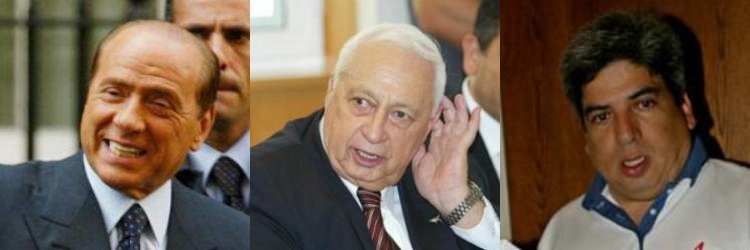
\includegraphics[width=10cm]{emp_studies/fd_failed}
		\caption{False negatives of the face dataset}
		\label{fig:failed_detection}
	\end{figure}



%███████╗██╗  ██╗██████╗ ███████╗██████╗        ██████╗ 
%██╔════╝╚██╗██╔╝██╔══██╗██╔════╝██╔══██╗       ╚════██╗
%█████╗   ╚███╔╝ ██████╔╝█████╗  ██████╔╝        █████╔╝
%██╔══╝   ██╔██╗ ██╔═══╝ ██╔══╝  ██╔══██╗       ██╔═══╝ 
%███████╗██╔╝ ██╗██║     ███████╗██║  ██║██╗    ███████╗
%╚══════╝╚═╝  ╚═╝╚═╝     ╚══════╝╚═╝  ╚═╝╚═╝    ╚══════╝
                                                       

\section{Experiment 2: Effectiveness of CNNs for Face Recognition}
	\subsection{Objective}
	Convolutional Neural Networks are used in many current state-of-art tools for face recognition (\cite{facenet_article}) and it is because their features why they were selected for this project. However, an analysis of how well does our network work specifically is something that must be present in this \gls{fyp}. 

	In this experiment, we test the network trained for the application and based in one of the models provided in \cite{facenet_github}. The network will be used to evaluate a set of images composed of an equal proportion of, on the one hand, face images extracted from the \gls{lfw} dataset and, on the other hand, face images of the author (\gls{mset} onwards), Mario Sánchez García. The two possible outputs of the evaluation will depend whether the author was recognised in the image or not. At the end, it is included an analysis of the results, including the \gls{mset} faces that were recognised, the \gls{mset} faces that were missed (i.e. false negatives) and the "random" faces that were recognised as the author (i.e. false positives). 

	\subsection{Method and parameters}
	The computer used is the same as the previous experiment, a Toshiba laptop model C50-A-1GU, with a 2,40 GHz Intel Processor Core i3-4000M, 8GB 1600MHz RAM memory and Kubuntu 17.10 OS (Linux kernel version 4.13.0-38-generic). 

	The face recognition is performed using the Tensorflow library. In fact, the code used here is exactly the same code included in the \textit{face{\_}recognition} module, already explained in the Design chapter (\ref{subsec:face_recog}). The \textit{main} function is adapted to train or evaluate the network using the data from the \gls{lfw} dataset, so the datasets must use its same format. This means that we have to create a folder "img" and then another folder inside to store all the images. The name of the last folder must be the class name of the subject, which in this case is "17226163". 

	The output of the face recognition process are rows with the following pattern: "X $<$class name$>$: Y.YYY". "X" is an integer that acts as the identifier of the image, starting from 0 and being incremented by 1 for each image. "Y.YYY" is a float from 0 to 1 with three digits of precission, which identify the confidence value of if the person identified is actually the person who appears in the image. The confidence value above which the identification was assumed to have been correct is 90\%.

	\subsection{Data set}
	The dataset used in the experiment is composed of a total of 80 face images, where 40 of these images (LFW-dataset onwards) has been manually obtained from the \gls{lfw} dataset and the other 40 images (i.e. \gls{mset}) are photos of the author. The Figure \ref{fig:fr_dataset} contains the complete dataset. 

	\begin{figure}[!ht]
		\centering
		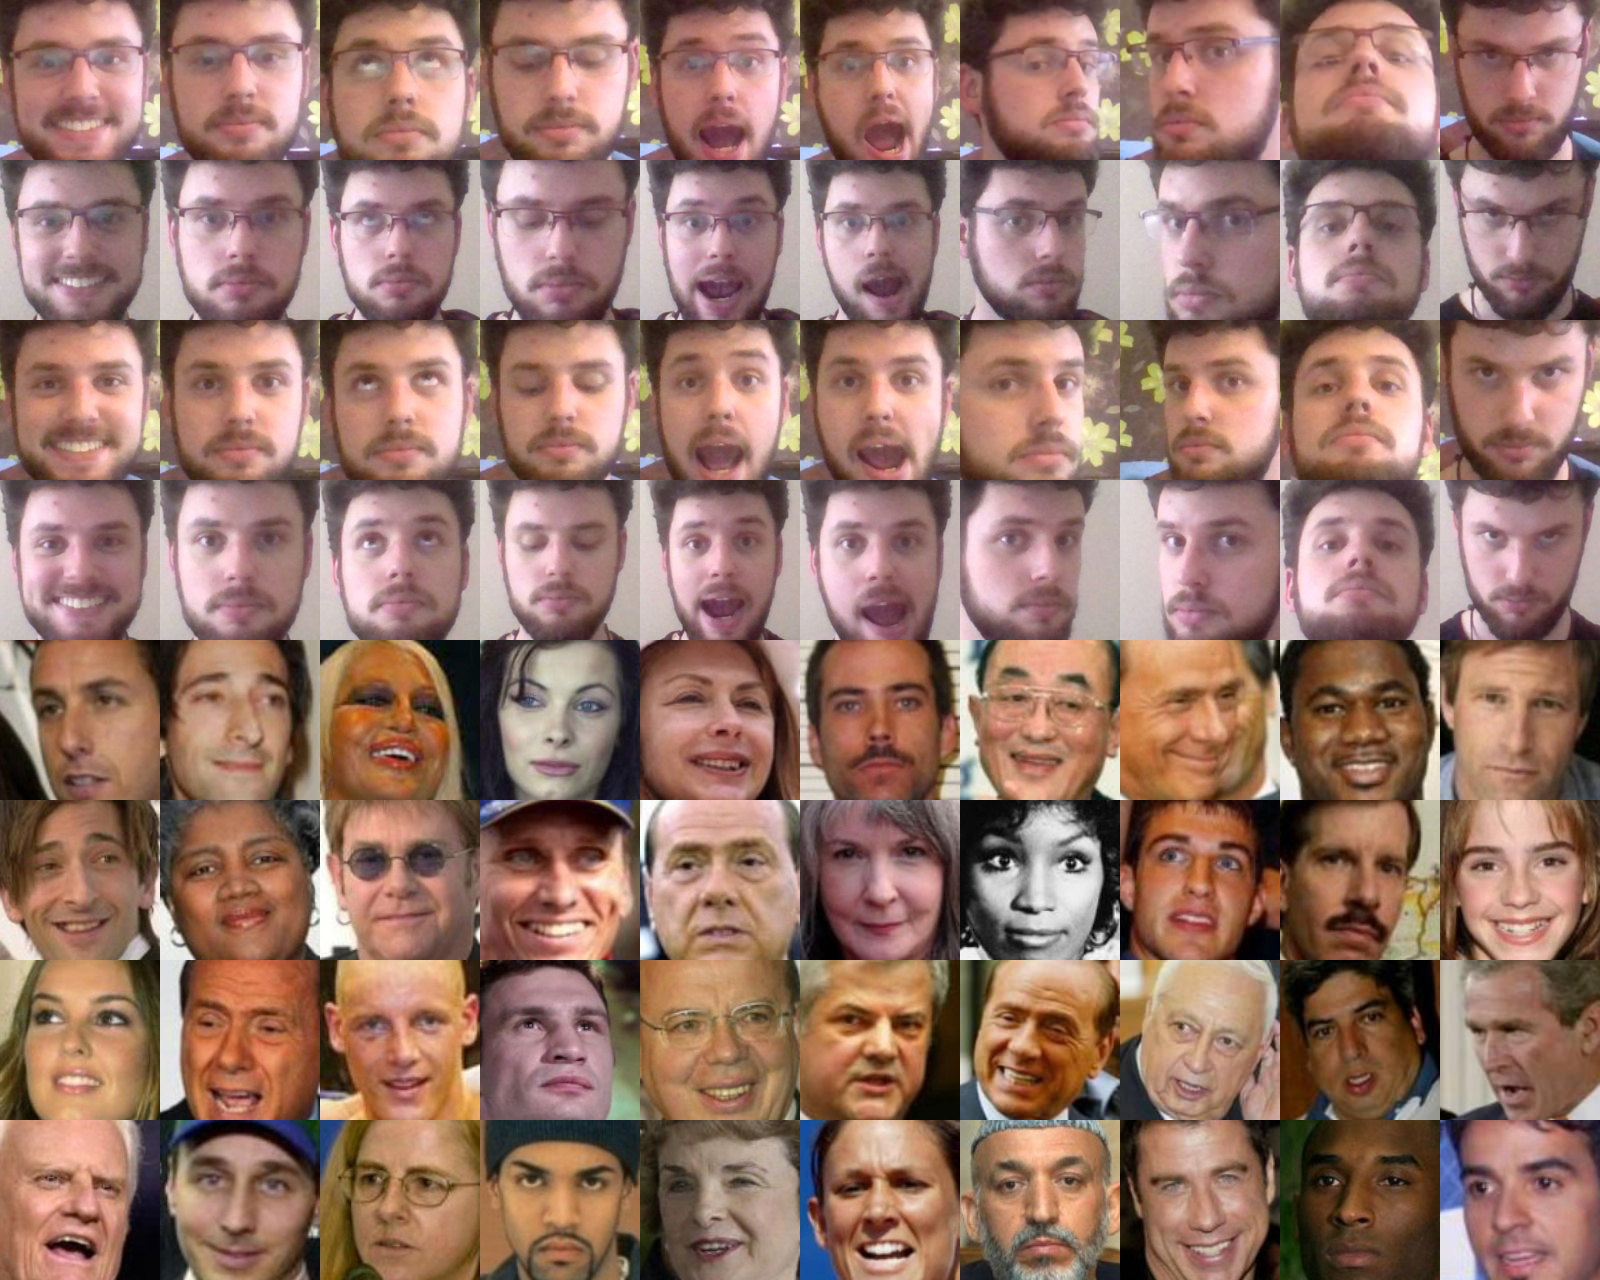
\includegraphics[width=14cm]{emp_studies/fr_dataset}
		\caption{Dataset for the Experiment 2}
		\label{fig:fr_dataset}
	\end{figure}

	All images are square-shaped with a resolution of 160x160 pixels. They have been pre-processed using the \textit{face{\_}detection} module, discussed in the Design chapter (\ref{subsec:face_det}), so they contain only the face of the person with a minimal background. The images in which no faces were detechttps://www.linguee.es/espanol-ingles/traduccion/esta+contemplado.htmlhttps://www.linguee.es/espanol-ingles/traduccion/esta+contemplado.htmlhttps://www.linguee.es/espanol-ingles/traduccion/esta+contemplado.htmlhttps://www.linguee.es/espanol-ingles/traduccion/esta+contemplado.htmlted were cropped manually simulating the pre-processing.

	The \gls{mset} is going to be explained in detail because a decision was made as to which photos to take. It is composed of 4 groups of images in which the illumination and the fact that the author wear glasses or not is varied:

	\begin{itemize}
		\item First group (Images 1-10). The light comes from the right and the author wear glasses.
		\item Second group (Images 11-20). The light comes from the left and the author wear glasses.
		\item Third group (Images 21-30). The light comes from the right and the author do not wear glasses.
		\item Fourth group (Images 31-40). The light comes from the left and the author do not wear glasses.
	\end{itemize}

	Within each group, the subject adopt in order the following poses or gestures: smiling, looking straight to the camera, looking up (eyes only), looking down (eyes only), mouth open, mouth open to the right, looking to the right, looking to the left, looking up (whole head), looking down (whole head).

	\subsection{Results}
	The exact results are included in the Tables \ref{table:results_exp2_mset} and \ref{table:results_exp2_lfwset} and can be seen in the Figures \ref{plot:results_exp2_mset} and \ref{plot:results_exp2_lfwset}, where a red line indicates the 90\% of confidence necessary to assume the recognition.

	\vspace{2cm}

	\begin{figure}[!ht]
		\centering
		\resizebox{\textwidth}{!}
		{		
			\begin{tikzpicture}
				\begin{axis}[
				    ybar, ymin=0, ymax=1, ylabel=Confidence,
				    x=0.5cm,
				    bar width=0.3cm,
				    enlarge x limits={abs=0.5cm},
				    xlabel=Image ID,
				    xtick=data,
				    xticklabels from table={exp2_mset_results.csv}{ImageID},
				    legend pos=south east,
				    tick style={
						grid=major,
						tick label style={rotate=45}
					}
				    ]
				    \addplot table [x expr=\coordindex, y=mset]{exp2_mset_results.csv};
				    \draw[red] (axis cs:-1,0.9) -- node[left]{} (axis cs:40,0.9);
				    \legend{M-dataset}
				\end{axis}
			\end{tikzpicture} 
		}
		\caption{Plot of the results (\gls{mset}) of the Experiment 2}
		\label{plot:results_exp2_mset}
	\end{figure}

	\vspace{2cm}

	\begin{figure}[!ht]
		\centering
		\resizebox{\columnwidth}{!}
		{		
			\begin{tikzpicture}
				\begin{axis}[
				    ybar, ymin=0, ymax=1, ylabel=Confidence,
				    x=0.5cm,
				    bar width=0.3cm,
				    enlarge x limits={abs=0.5cm},
				    xlabel=Image ID,
				    xtick=data,
				    xticklabels from table={exp2_lfwset_results.csv}{ImageID},
				    legend pos=south east,
				    tick style={
						grid=major,
						tick label style={rotate=45} 
					}
				    ]
				    \addplot[red,fill=red!30!white] table [x expr=\coordindex, y=lfwset]{exp2_lfwset_results.csv};
				    \draw[red] (axis cs:-1,0.9) -- node[left]{} (axis cs:40,0.9);
				    \legend{LFW-dataset}
				\end{axis}
			\end{tikzpicture} 
		}
		\caption{Plot of the results (LFW-dataset) of the Experiment 2}
		\label{plot:results_exp2_lfwset}
	\end{figure}

	\clearpage

	\begin{adjustwidth}{-0.5in}{-0.4in}
	\renewcommand{\arraystretch}{0.9}
	\begin{multicols}{2}

		\begin{table}[H]
			\centering
		    \resizebox{!}{9.5cm}
			{		
		    \begin{tabular}{| C{2.3cm} | R{2.3cm} | C{2.3cm} |}
			    \hline
			    Image ID 	& \multicolumn{1}{c|}{Confidence}  	& Recognised 	\\ \hline
					0		&			95.4\%					& \checkmark	\\ \hline  
					1		&			96.4\%					& \checkmark	\\ \hline  
					2		&			94.6\%					& \checkmark	\\ \hline  
					3		&			95.7\%					& \checkmark	\\ \hline  
					4		&			96.9\%					& \checkmark	\\ \hline  
					5		&			96.9\%					& \checkmark	\\ \hline  
					6		&			92.3\%					& \checkmark	\\ \hline  
					7		&			92.6\%					& \checkmark	\\ \hline  
					8		&			96.0\%					& \checkmark	\\ \hline  
					9		&			93.6\%					& \checkmark	\\ \hline  
					10		&			93.0\%					& \checkmark	\\ \hline 
					11		&			95.7\%					& \checkmark	\\ \hline 
					12		&			90.6\%					& \checkmark	\\ \hline 
					13		&			92.2\%					& \checkmark	\\ \hline 
					14		&			96.0\%					& \checkmark	\\ \hline 
					15		&			91.1\%					& \checkmark	\\ \hline 
					16		&			92.9\%					& \checkmark	\\ \hline 
					17		&			88.6\%					& \xmark		\\ \hline 
					18		&			94.4\%					& \checkmark	\\ \hline 
					19		&			80.8\%					& \xmark		\\ \hline 
					20		&			95.0\%					& \checkmark	\\ \hline 
					21		&			95.6\%					& \checkmark	\\ \hline 
					22		&			95.9\%					& \checkmark	\\ \hline 
					23		&			94.3\%					& \checkmark	\\ \hline 
					24		&			84.3\%					& \xmark		\\ \hline 
					25		&			94.2\%					& \checkmark	\\ \hline 
					26		&			94.3\%					& \checkmark	\\ \hline 
					27		&			94.4\%					& \checkmark	\\ \hline 
					28		&			94.9\%					& \checkmark	\\ \hline 
					29		&			95.9\%					& \checkmark	\\ \hline 
					30		&			96.1\%					& \checkmark	\\ \hline 
					31		&			92.3\%					& \checkmark	\\ \hline 
					32		&			95.0\%					& \checkmark	\\ \hline 
					33		&			95.2\%					& \checkmark	\\ \hline 
					34		&			94.0\%					& \checkmark	\\ \hline 
					35		&			96.1\%					& \checkmark	\\ \hline 
					36		&			92.4\%					& \checkmark	\\ \hline 
					37		&			95.5\%					& \checkmark	\\ \hline 
					38		&			95.1\%					& \checkmark	\\ \hline 
					39		&			95.1\%					& \checkmark	\\ \hline 					 			 
			\end{tabular}
		    }
			\caption{Results of \gls{mset} in the Experiment 2}
		    \label{table:results_exp2_mset}
		\end{table}
 
		\begin{table}[H]
			\centering
		    \resizebox{!}{9.5cm}
			{		
		    \begin{tabular}{| C{2.3cm} | R{2.3cm} | C{2.3cm} |}
			    \hline
			    Image ID 	& \multicolumn{1}{c|}{Confidence}  	& Recognised \\ \hline
					40 		&			25.1\%					& \xmark	 \\ \hline
					41 		&			22.0\%					& \xmark	 \\ \hline
					42 		&			22.1\%					& \xmark	 \\ \hline
					43 		&			37.6\%					& \xmark	 \\ \hline
					44 		&			27.9\%					& \xmark	 \\ \hline
					45 		&			33.7\%					& \xmark	 \\ \hline
					46 		&			27.1\%					& \xmark	 \\ \hline
					47 		&			37.8\%					& \xmark	 \\ \hline
					48 		&			38.4\%					& \xmark	 \\ \hline
					49 		&			18.3\%					& \xmark	 \\ \hline
					50 		&			21.4\%					& \xmark	 \\ \hline
					51 		&			35.0\%					& \xmark	 \\ \hline
					52 		&			34.3\%					& \xmark	 \\ \hline
					53 		&			34.9\%					& \xmark	 \\ \hline
					54 		&			43.2\%					& \xmark	 \\ \hline
					55 		&			29.4\%					& \xmark	 \\ \hline
					56 		&			32.7\%					& \xmark	 \\ \hline
					57 		&			38.3\%					& \xmark	 \\ \hline
					58 		&			69.9\%					& \xmark	 \\ \hline
					59 		&			28.4\%					& \xmark	 \\ \hline
					60 		&			25.1\%					& \xmark	 \\ \hline
					61 		&			20.0\%					& \xmark	 \\ \hline
					62 		&			31.1\%					& \xmark	 \\ \hline
					63 		&			49.0\%					& \xmark	 \\ \hline
					64 		&			31.7\%					& \xmark	 \\ \hline
					65 		&			32.5\%					& \xmark	 \\ \hline
					66 		&			23.6\%					& \xmark	 \\ \hline
					67 		&			40.5\%					& \xmark	 \\ \hline
					68 		&			79.3\%					& \xmark	 \\ \hline
					69 		&			29.9\%					& \xmark	 \\ \hline
					70 		&			41.3\%					& \xmark	 \\ \hline
					71 		&			22.3\%					& \xmark	 \\ \hline
					72 		&			25.8\%					& \xmark	 \\ \hline
					73 		&			47.5\%					& \xmark	 \\ \hline
					74 		&			68.8\%					& \xmark	 \\ \hline
					75 		&			50.5\%					& \xmark	 \\ \hline
					76 		&			25.8\%					& \xmark	 \\ \hline
					77 		&			28.1\%					& \xmark	 \\ \hline
					78 		&			48.0\%					& \xmark	 \\ \hline
					79 		&			39.3\%					& \xmark	 \\ \hline
			\end{tabular}
		    }
			\caption{Results of LFW-dataset in the Experiment 2}
		    \label{table:results_exp2_lfwset}
		\end{table}

	\end{multicols}
	\renewcommand{\arraystretch}{1}
	\end{adjustwidth}

	\subsection{Evaluation}
	In this section we will evaluate the results shown previously. In the Table \ref{table:true_false_exp2} we can find a brief analysis of the data, showing the false positives and negatives.

	\begin{table}[H]
		\centering
		    \begin{tabular}{L{2.5cm} | R{2cm} | R{2cm} |}
			    \cline{2-3}
			    & \multicolumn{1}{c|}{Positive} & \multicolumn{1}{c|}{Negative}\\ 
			    \hline
			    \multicolumn{1}{|c|}{True} 	& 37 	& 40 \\
				\hline
				\multicolumn{1}{|c|}{False} &  0 	&  3 \\
				\hline
			\end{tabular}
		\caption{Analysis of results of the Experiment 2}
	    \label{table:true_false_exp2}
	\end{table}

	As we did in the previous experiment, we are going to use the metrics of \textit{precision} and \textit{recall}.

	\begin{flalign}
		\label{eq:prec_exp2}
		Precission  &= \frac{relevant \cap retrieved}{retrieved} = \\ \nonumber
					&= \frac{positive_{true}}{positive_{true} \cup positive_{false}} = \frac{37}{37+0} = 100\%
	\end{flalign}

	\begin{flalign}
		\label{eq:recall_exp2}
		Recall 	&= \frac{relevant \cap retrieved}{relevant} = \\\nonumber
				&= \frac{positive_{true}}{positive_{true} \cup negative_{false}} = \frac{37}{37+3} = 92.5\%
	\end{flalign}

	With a 100\% of precision and 92.5\% of recall, we can see the huge potential of the Convolutional Neural Networks for face recognition, even with variations in pose, gesture, illumination and accessories (e.g. glasses). From the \gls{lfw} dataset none of the faces were recognised, not only as the author, but neither as any of the other "students" (in fact, different subjects also from the \gls{lfw}) for who the network was trained. The highest confidence value of this dataset was 79.3\%, not even close to the necessary 90\%.

	\clearpage

	About the false negatives, the three photos were rejected because they did not exceed the selected confidence level of 90\%, but with more than 80\% in all of them, the identification of the author was almost confirmed. One option would be to lower this value to, say, 80\%. However, the use of this application tolerate better the false negatives than the false positives, which could have occurred with an 80\%, so the confidence value will be kept at 90\%. 

	In the case of a false positive, the user would be recognised as another student and would have to wait for the \textit{timetable} and \textit{map} calls to the server to know that in fact, from the beginning, the information is not valid. On the other hand, in the case of a false negative, the Error window would show up after the failed recognition, allowing the user to repeat the process much faster.
	